\section{Other Work}

In this section we will discuss some of the work that has come out since AlphaZero. There have been a number of improvements as well as an increased theoretical understanding. This will not be an exhaustive treatment of the work and is only intended to give the reader a taste of what is out there in the hopes that will make further pursuit of these topics easier. It will not be exhaustive in depth or in breadth. There is more work being produce seemingly all the time that builds on top of what we have discussed in this paper. 

\subsection{MuZero}

Recall that while training a AlphaGo algorithm you need a model of the environment. In order to perform MCTS you have to have an accurate model of the environment that is capable of giving you the next state given a current state and action. The environment also needs to tell you when the game has ended and what the associated reward is. This is a barrier for being able to apply the concepts learned in ALphaGo to other domains. In 2019 Deepmind released a paper \cite{muzero} that helped to address these issues. The algorithm has many similarities to AlphaZero and so lets look at where it differs. MuZero performs MCTS in a latent space with a learned model. That is as they are performing each step of MCTS in a state space that is not directly representative of an actual state in the environment. Let look at a figure of this to see what I mean. 

\begin{figure}[H]
       \centering
       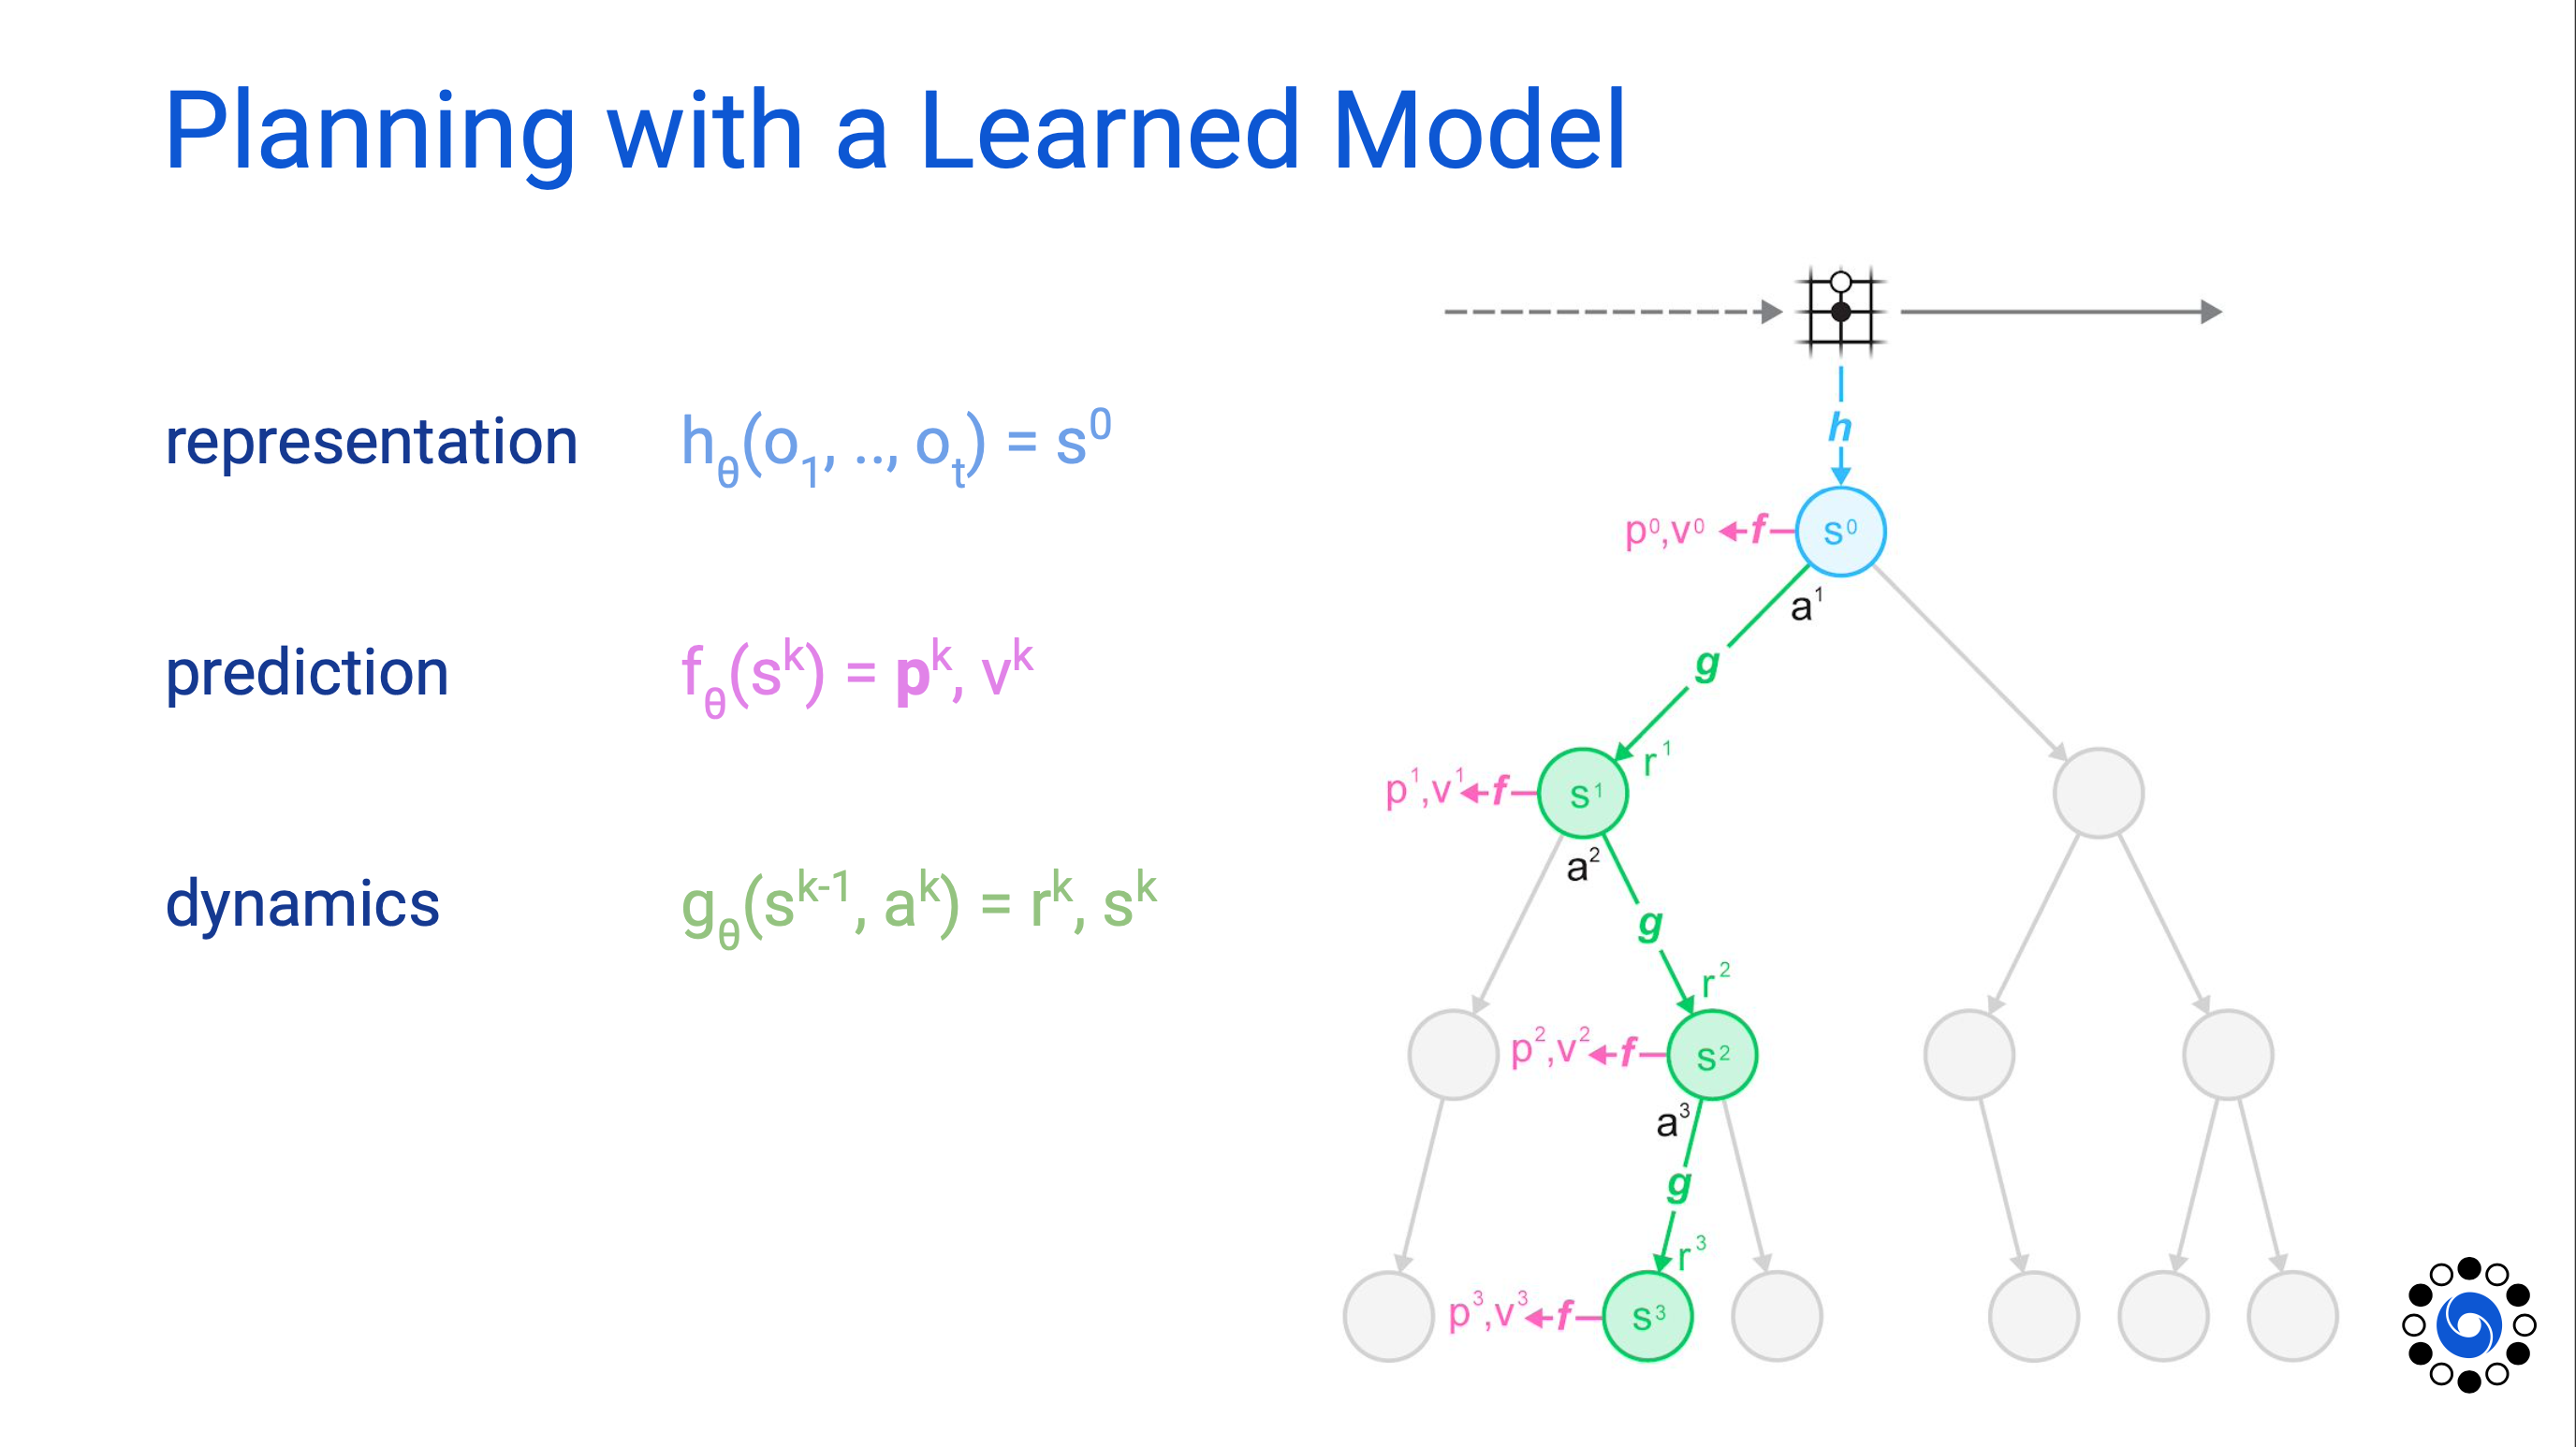
\includegraphics[width=400px,height=200px]{images/muzero_learned_model.png}
       \caption{Planning in MuZero}
       \label{fig:my_label}
\end{figure}

The current state of the environment is used for the root node as usual except now there is a \textbf{representation} network that takes the environment state and produces a vector representation of that state in a latent space. From this new space you need to run all the normal MCTS except without a model. This is achieved by learning a dynamics model that sits in place of the true environment. The interesting thing is that this dynamics model is not learned by attempting to make it be able to model the true environment more and more accurately which is the standard approach. Here the dynamics model is learned so as to maximize reward (more to come on reward). The idea is that in some cases it might not be necessary and even detrimental to plan with the true model. From the figure you can see that the dynamics function takes in a state action pair and produces the next state and reward. This means that they are also learning a representation for reward. This has the flexibility of potentially learning intermediate reward states. There is still a network that outputs a policy and a value from a given state represented in the figure as the \textbf{prediction} $f_\theta$. Since there is no environment to tell the search when its hit a leaf node they just search for a predefined set of steps. The hope is that the dynamics will start to treat leaf nodes as a sort of steady state and if it is asked to predict the next state past a leaf node then it will output the same reward and state as it was just in. The result of the search is as before with a distribution over possible actions. 

The data generated during training is similar as before. The figure below gives more of a birds eye view of the training loop. In part \textbf{B} we see that MuZero acts in the real environment in a similar matter as before. MuZero samples from the policy distribution given by the search. The environment than provides the next state which is fed into the search. For training the network a trajectory of state action pairs is sampled from the replay buffer. This is different from AlphaZero that just samples state action pairs randomly and not necessarily as a trajectory. This is necessary because to learn the dynamics model we actually feed in actions from the trajectory. The dynamics network is "unrolled" for K hypothetical steps and the output is used to train the network. As mentioned before there are 3 different networks and that means three different loss functions. They are trained jointly using backpropagation through time. The policy network is made to more closely resemble the output that is given by search. The reward output from the dynamics function is made to more closely match what is given by the true environment. The value function is trained to predict the result of the sample return. The

\begin{equation}
    l_{t}(\theta) = \sum_{k=0}^{K} l^{r}(u_{t + k},r_{t}
\end{equation}


\begin{figure}[H]
       \centering
       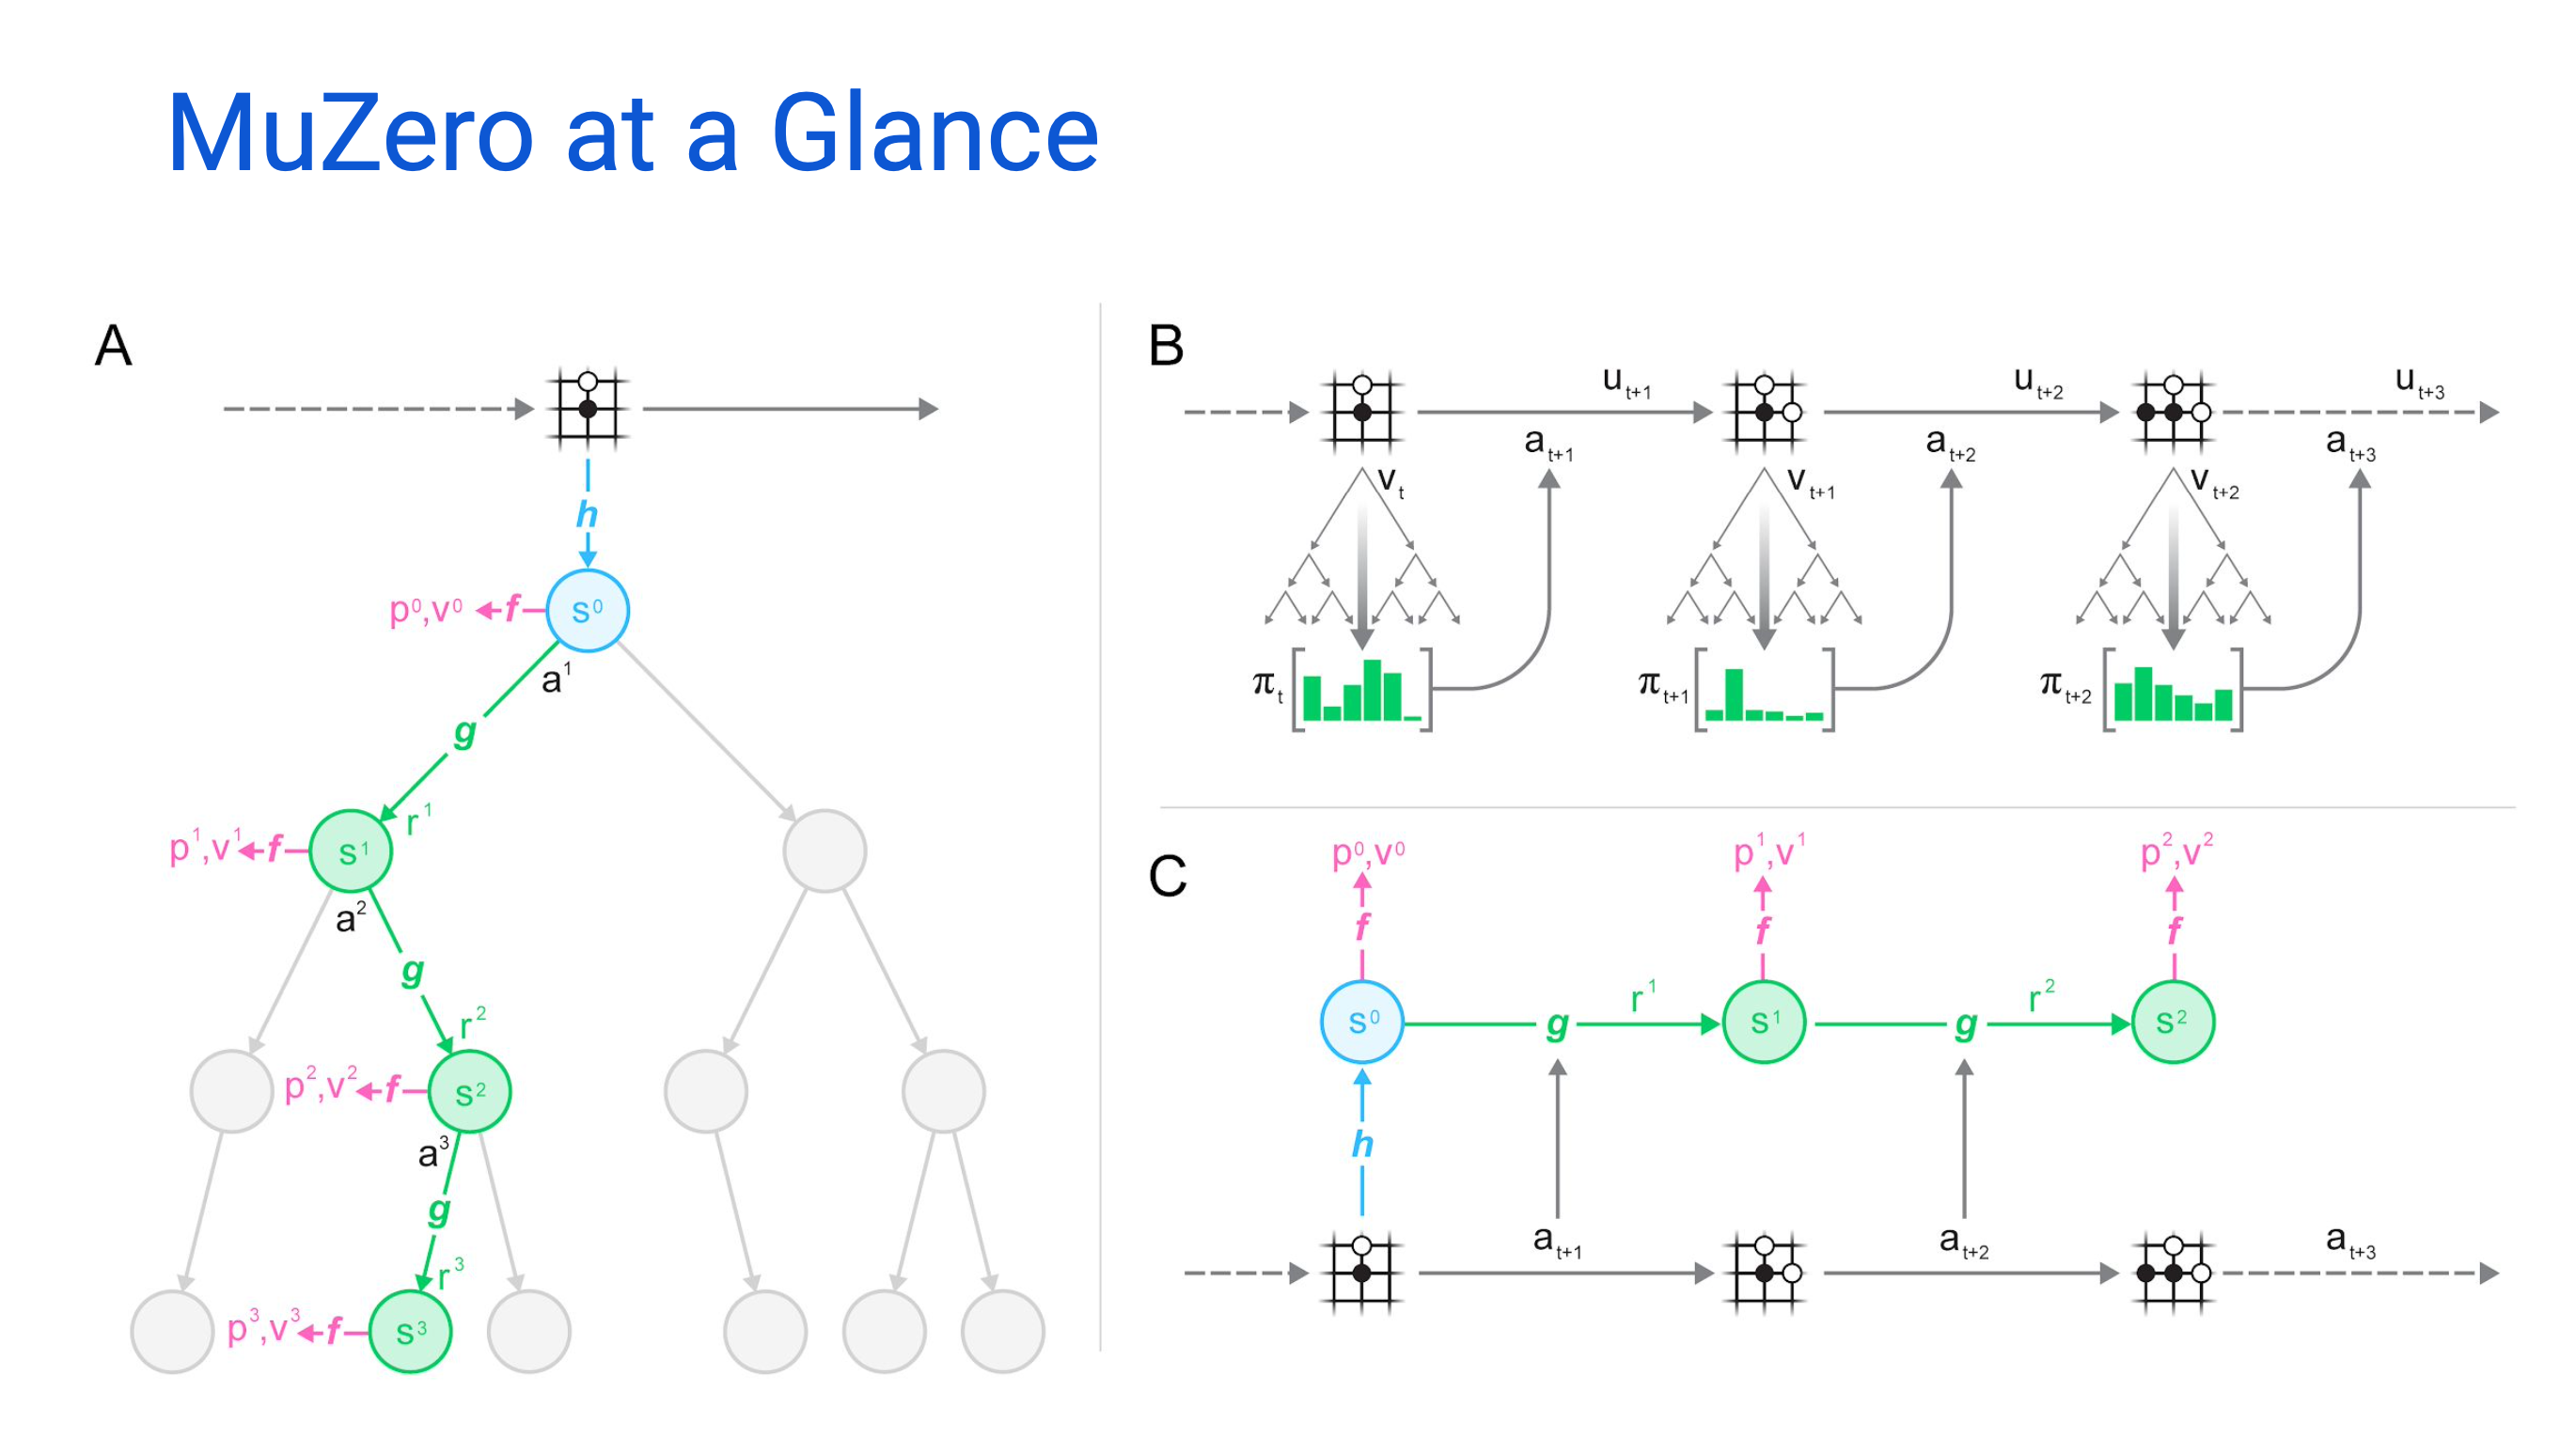
\includegraphics[width=400px,height=200px]{images/muzero_planning.png}
       \caption{Planning in MuZero}
       \label{fig:my_label}
\end{figure}


\subsection{MCTS as regularized policy optimization}

A paper by Jean-Bastien Grill and colleagues #TODO [Citation] proposed to show in rigorous detail the theoretical understanding for what AlphaZero actually is. They show that AlphaZero and similar MCTS based algorithms are really approximations to a regularized policy optimization problem. They also show that it is possible to find the exact solution and use that as a replacement for AlphaZero and obtain better results. I think that this was a fantastic paper and will really help you understand AlphaZero if you take the time to go through it. Lets look at some of the highlights of the paper. 

First it is necessary to understand what \textbf{policy optimization} is. This is an approach to solving RL type problems by directly maximizing reward by looking at the gradient of your loss function w.r.t the parameters of your policy network. So the optimal policy is obtained by incrementally improving the policy network directly. The regularized version of this concept is discussed in the current paper. Here is the maximization problem that is trying to be solved.

\begin{equation}
    \pi_{\theta^{'}} \overset{\triangle}{=} \underset{y \epsilon S}{arg \ max} Q_{\pi_{\theta}}^{T}\y - R(y,\pi_{\theta})
\end{equation}

Q is the same Q function that we have seen in AlphaZero. The subscript just means that it is a value estimate w.r.t a certain policy. \textbf{y} is a vector that represents the action distribution that we are looking for to maximize the equation. $R(y,\pi_\theta)$ is a regularization term. Their main claim in this paper is that the selection criterion use by AlphaZero "can be interpreted as approximating the solution to a regularized policy-optimization objective". Some notation will be needed to understand the core concepts of the paper. First they define a multiplier that is used to help simplify some expressions. 

\begin{equation}
    \lambda_{N} (s) \overset{\triangle}{=} c * \frac{\sqrt{\sum_{b}n_{b}}}{|\mathbf{A}| + \sum_{b}n_{b}}
\end{equation}

Most of these terms we have seen alread. $| \mathbf{A} |$ is the number of possible actions in the given domain and $n_{b}$ is the number of times a particular node has been visited. $c$ is the $puct$ constant. This allows them to rewrite the MCTS select criterion. 

\begin{equation}
    a^{*} \overset{\triangle}{=} arg \ max [\textbf{q} + \lambda_{N} \frac{\pi_{\theta}}{\hat{\pi}}]
\end{equation}

Here $\textbf{q} = Q(s,a)$ and $ \pi_{\theta} = \pi_{\theta}(a | s)$ the policy distribution from our network and $\hat{\pi}$ is the policy distribution given by MCTS. They show that $\hat{\pi}$ is an approximation to a solution (${\bar{\pi}}$) of a regularized policy optimization problem.

\begin{equation}
    \bar{\pi} \overset{\triangle}{=} \underset{y \epsilon S}{arg \ max} \ \textbf{q}^{T}\y - \lambda_{N}KL(\pi_{\theta},y)
\end{equation}

Here the regularization term is KL-divergence and is in reverse of how it is normally written. They show that $\hat{\pi}$ actually tracks $\bar{\pi}$. They also show how the MCTS UCT that we looked at early in this paper is actually approximating a similar $\bar{\pi}$ but with a different regularization term. They then describe why just calculating $\bar{\pi}$ directly is preferable. Since $\bar{\pi}$ can be substituted in place of $\hat{\pi}$ you can just swap out one for the other in any place that it is used. In AlphaZero $\hat{\pi}$ is used in three places. It is used in selecting actions, during search and also when training the network. 

To demonstrate the applicability of their approach they ran a series of experiments using MuZero as a baseline. The first figure below helps demonstrate that MuZero is indeed approximating their algorithm and also the large impact that the number of simulations has on performance for MuZero. "All" in this figure stands for the fact that they swapped in $\bar{\pi}$ for each one of the three steps that were mentioned above. We can see that especially for a small number of simulations "All" vastly outperforms MuZero but they converge to equal performance as the simuations are increased. 

\begin{figure}[H]
       \centering
       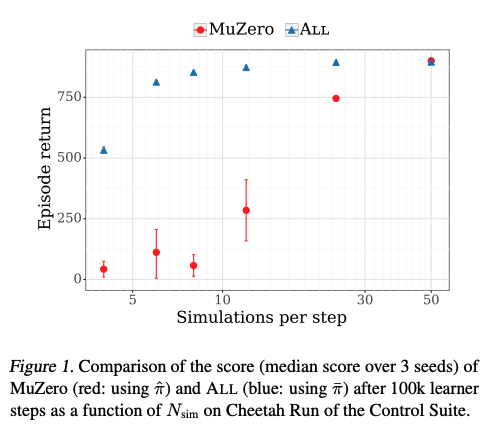
\includegraphics[width=400px,height=200px]{experiments/mcts_reg_figure_1.png}
       \label{fig:my_label}
\end{figure}

They performed experiments a number of Atari games and seem to demonstrate quite definitively the performance gains achieved using their method. This paper is quite impressive and well worth your time to go and read it if you want to have a deeper understanding of AlphaZero.  


\begin{figure}[H]
       \centering
       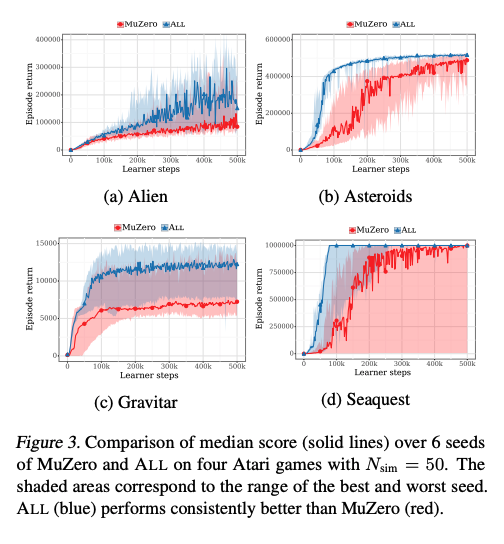
\includegraphics[width=400px,height=200px]{experiments/mcts_reg_figure_3.png}
       \label{fig:my_label}
\end{figure}

\subsection{Other work and applications AlphaZero}

I will just point the reader at a few papers that extend ALphaZero or use it in a novel way. There is many more I am sure at this point as the literature continues to expand at a rapid pace in this area. 

\begin{itemize}
    \item AlphaZero is intended to work in domains in which the action space is discrete. Extending the work to continous actions space would greatly help in being able to use it in "real" world applications such as robotics.
    \textbf{A0C: Alpha Zero in Continuous Action Space}
    \cite{aocalphazero}
    
    \item \textbf{Improved protein structure prediction using potentials from deep learning}
    \cite{alphafold}
    
    \item \textbf{TOWARDS “ALPHA CHEM”: CHEMICAL SYNTHESIS PLANNING WITH TREE SEARCH AND
    DEEP NEURAL NETWORK POLICIES}
    \cite{alphachem}
    
    \item Optimizing quantum dynamics
    \textbf{Dalgaard, Mogens, et al. "Global optimization of quantum dynamics with AlphaZero deep exploration." npj Quantum Information 6.1 (2020).}
    \cite{alphaquantum} 
    
\end{itemize}

